\documentclass[oneside,a4paper,14pt]{extarticle}
\usepackage[T1,T2A]{fontenc}
\usepackage[
a4paper,
letterpaper,
top=2cm,
bottom=2cm,
left=2.5cm,
right=1.5cm
]{geometry}
\usepackage[utf8]{inputenc}
\usepackage[russian]{babel}
\usepackage{textcomp}
\usepackage{indentfirst}
\usepackage{listings}
\usepackage{xcolor}
\usepackage{enumitem}
\usepackage{graphicx}
\usepackage{mwe}
\usepackage{wrapfig}
\usepackage{caption}
\usepackage{amsmath}
\usepackage{amsfonts}
\usepackage{float}
\usepackage{amsthm}
\usepackage[all]{xy}
\usepackage[breaklinks]{hyperref}
\usepackage{titlesec}
\usepackage{adjustbox} % <-- ДОБАВЛЕН ПАКЕТ ДЛЯ ОГРАНИЧЕНИЯ РАЗМЕРА
\titleformat{\section}
{\normalsize\bfseries}
{\thesection} {1em}{}
\titleformat{\subsection}
{\normalsize\bfseries}
{\thesubsection} {1em}{}
\titleformat{\subsubsection}
{\normalsize\bfseries}
{\thesubsubsection} {1em}{}
\renewcommand\baselinestretch{1.33}
\normalsize
\setlength{\parindent}{1.25cm}
\lstset{
	language=SQL,
	basicstyle=\ttfamily\small,
	keywordstyle=\color{blue},
	commentstyle=\color{green!60!black},
	stringstyle=\color{red},
	numbers=left,
	numberstyle=\tiny\color{gray},
	frame=single,
	breaklines=true,
	showstringspaces=false,
	tabsize=4,
	inputencoding=utf8,
	extendedchars=true,
	literate={а}{{\selectfont\char224}}1 {б}{{\selectfont\char225}}1 {в}{{\selectfont\char226}}1 {г}{{\selectfont\char227}}1 {д}{{\selectfont\char228}}1 {е}{{\selectfont\char229}}1 {ж}{{\selectfont\char230}}1 {з}{{\selectfont\char231}}1 {и}{{\selectfont\char232}}1 {й}{{\selectfont\char233}}1 {к}{{\selectfont\char234}}1 {л}{{\selectfont\char235}}1 {м}{{\selectfont\char236}}1 {н}{{\selectfont\char237}}1 {о}{{\selectfont\char238}}1 {п}{{\selectfont\char239}}1 {р}{{\selectfont\char240}}1 {с}{{\selectfont\char241}}1 {т}{{\selectfont\char242}}1 {у}{{\selectfont\char243}}1 {ф}{{\selectfont\char244}}1 {х}{{\selectfont\char245}}1 {ц}{{\selectfont\char246}}1 {ч}{{\selectfont\char247}}1 {ш}{{\selectfont\char248}}1 {щ}{{\selectfont\char249}}1 {ъ}{{\selectfont\char250}}1 {ы}{{\selectfont\char251}}1 {ь}{{\selectfont\char252}}1 {э}{{\selectfont\char253}}1 {ю}{{\selectfont\char254}}1 {я}{{\selectfont\char255}}1 {А}{{\selectfont\char192}}1 {Б}{{\selectfont\char193}}1 {В}{{\selectfont\char194}}1 {Г}{{\selectfont\char195}}1 {Д}{{\selectfont\char196}}1 {Е}{{\selectfont\char197}}1 {Ж}{{\selectfont\char198}}1 {З}{{\selectfont\char199}}1 {И}{{\selectfont\char200}}1 {Й}{{\selectfont\char201}}1 {К}{{\selectfont\char202}}1 {Л}{{\selectfont\char203}}1 {М}{{\selectfont\char204}}1 {Н}{{\selectfont\char205}}1 {О}{{\selectfont\char206}}1 {П}{{\selectfont\char207}}1 {Р}{{\selectfont\char208}}1 {С}{{\selectfont\char209}}1 {Т}{{\selectfont\char210}}1 {У}{{\selectfont\char211}}1 {Ф}{{\selectfont\char212}}1 {Х}{{\selectfont\char213}}1 {Ц}{{\selectfont\char214}}1 {Ч}{{\selectfont\char215}}1 {Ш}{{\selectfont\char216}}1 {Щ}{{\selectfont\char217}}1 {Ъ}{{\selectfont\char218}}1 {Ы}{{\selectfont\char219}}1 {Ь}{{\selectfont\char220}}1 {Э}{{\selectfont\char221}}1 {Ю}{{\selectfont\char222}}1 {Я}{{\selectfont\char223}}1,
}
\begin{document}
	\newpage\thispagestyle{empty}
	\begin{center}
		МИНИСТЕРСТВО НАУКИ И ВЫСШЕГО ОБРАЗОВАНИЯ\\
		РОССИЙСКОЙ ФЕДЕРАЦИИ\\
		ФЕДЕРАЛЬНОЕ ГОСУДАРСТВЕННОЕ БЮДЖЕТНОЕ\\
		ОБРАЗОВАТЕЛЬНОЕ УЧРЕЖДЕНИЕ ВЫСШЕГО ОБРАЗОВАНИЯ\\
		<<ВЯТСКИЙ ГОСУДАРСТВЕННЫЙ УНИВЕРСИТЕТ>>\\
		Институт математики и информационных систем\\
		Факультет автоматики и вычислительной техники\\
		Кафедра электронных вычислительных машин
	\end{center}
	\vspace{20mm}
	\begin{center}
		Отчёт по лабораторной работе №2.2\\
		по дисциплине\\
		<<Базы данных>>\\
	\end{center}
	\vspace{48mm}
	\noindent
	Выполнил студент гр. ИВТб-2303-06-00 \hfill \rule[-0,5mm]{30mm}{0.15mm}\,/Шубин В. Ю./
	\newline
	Проверил преподаватель кафедры ЭВМ \hfill \rule[-0,5mm]{30mm}{0.15mm}\,/Клюкин В. Л./
	\vfill
	\begin{center}
		Киров\\
		2026
	\end{center}
	\newpage
	\thispagestyle{empty}
	\section*{Цель работы:} Научиться использованию агрегатных функций, операторов и встроенных функций, работе с датами, подзапросами и предложениями WITH, RETURNING. Рассмотреть и выполнить различные планы выполнения запросов, выполнить FORMAT JSON для выборки из нескольких связанных таблиц, выполнить три способа соединения для одной и той же выборки и определить наиболее оптимальный.
	
	\section*{Среда разработки:} PostgreSQL 18, pgAdmin 4, Windows 10.
	
	\newpage
	
	\section*{Агрегатные функции}
	
	\begin{lstlisting}
		-- s1: количество записей в таблице game
		SELECT count(*) FROM lab_schema.game;
		
		-- s2: сумма, минимум, максимум и средняя цена всех игр
		SELECT 
		sum(price) AS total_price,
		min(price) AS min_price,
		max(price) AS max_price,
		round(avg(price), 2) AS avg_price
		FROM lab_schema.game;
		
		-- s3: группировка - количество игр и средняя оценка по разработчику
		SELECT 
		d.name AS developer,
		count(g.id) AS games_count,
		round(avg(r.score), 2) AS avg_score
		FROM lab_schema.developer d
		JOIN lab_schema.game g ON g.developer_id = d.id
		JOIN lab_schema.review r ON r.game_id = g.id
		GROUP BY d.id, d.name
		ORDER BY avg_score DESC;
		
		-- s4: список жанров для каждой игры через string_agg
		SELECT 
		g.title AS game_title,
		string_agg(gen.name, ', ') AS genres
		FROM lab_schema.game g
		JOIN lab_schema.game_genre gg ON g.id = gg.game_id
		JOIN lab_schema.genre gen ON gg.genre_id = gen.id
		GROUP BY g.id, g.title;
		
		-- s5: HAVING - разработчики со средней оценкой > 8
		SELECT 
		d.name AS developer,
		round(avg(r.score), 2) AS avg_score
		FROM lab_schema.developer d
		JOIN lab_schema.game g ON g.developer_id = d.id
		JOIN lab_schema.review r ON r.game_id = g.id
		GROUP BY d.id, d.name
		HAVING avg(r.score) > 8
		ORDER BY avg_score DESC;
	\end{lstlisting}
	
	Результат выполнения запроса s1 представлен на рисунке~1.
	
	\begin{figure}[H]
		\centering
		\adjustbox{max width=\linewidth}{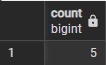
\includegraphics{s1.png}}
		\caption{Результат запроса s1}
	\end{figure}
	
	Результат выполнения запроса s2 представлен на рисунке~2.
	
	\begin{figure}[H]
		\centering
		\adjustbox{max width=\linewidth}{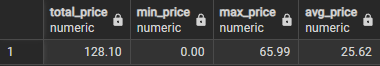
\includegraphics{s2.png}}
		\caption{Результат запроса s2}
	\end{figure}
	
	Результат выполнения запроса s3 представлен на рисунке~3.
	
	\begin{figure}[H]
		\centering
		\adjustbox{max width=\linewidth}{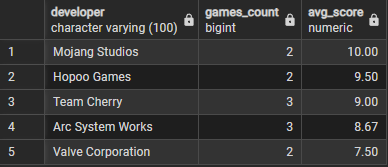
\includegraphics{s3.png}}
		\caption{Результат запроса s3}
	\end{figure}
	
	Результат выполнения запроса s4 представлен на рисунке~4.
	
	\begin{figure}[H]
		\centering
		\adjustbox{max width=\linewidth}{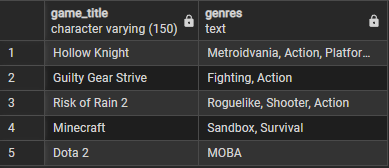
\includegraphics{s4.png}}
		\caption{Результат запроса s4}
	\end{figure}
	
	Результат выполнения запроса s5 представлен на рисунке~5.
	
	\begin{figure}[H]
		\centering
		\adjustbox{max width=\linewidth}{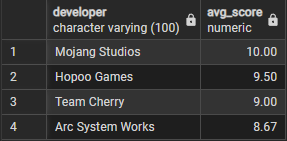
\includegraphics{s5.png}}
		\caption{Результат запроса s5}
	\end{figure}
	
	\newpage
	
	\section*{Операторы и встроенные функции}
	
	\begin{lstlisting}
		-- s6: логические операторы and, or, not
		SELECT NOT 1 < 2 AND 3 < 4 OR 5 = 5 AS result;
		
		-- s7: операторы IS NULL, IS NOT NULL
		SELECT 1 IS NULL OR 5 IS NOT NULL AS result;
		
		-- s8: BETWEEN - игры, вышедшие в диапазоне лет
		SELECT * FROM lab_schema.game 
		WHERE release_year BETWEEN 2015 AND 2022;
		
		-- s9: конкатенация строк через || и concat
		SELECT 
		title || ' by ' || d.name AS game_info,
		concat(title, ' (', release_year, ')') AS game_full
		FROM lab_schema.game g
		JOIN lab_schema.developer d ON g.developer_id = d.id;
		
		-- s10: разница между || и concat при работе с NULL
		SELECT 
		'abc' || NULL AS concat_operator,
		concat('abc', NULL, 'de') AS concat_func;
		
		-- s11: функции lower, upper, trim
		SELECT 
		lower('HOLLOW KNIGHT') AS lower_name,
		upper('dota') AS upper_name,
		trim('  Minecraft  ') AS trimmed;
		
		-- s12: CASE для категоризации игр по цене
		SELECT 
		title,
		price,
		CASE 
		WHEN price = 0 THEN 'Free-to-play'
		WHEN price < 20 THEN 'Budget'
		WHEN price < 40 THEN 'Standard'
		ELSE 'Premium'
		END AS price_category
		FROM lab_schema.game
		ORDER BY price;
		
		-- s13: COALESCE - первый не-NULL аргумент
		SELECT 
		title,
		COALESCE(country, 'Unknown') AS developer_country
		FROM lab_schema.game g
		JOIN lab_schema.developer d ON g.developer_id = d.id;
		
		-- s14: LIKE - поиск по шаблону
		SELECT * FROM lab_schema.game WHERE title LIKE '%Knight%';
		
		-- s15: приведение типов через ::
		SELECT 
		price::text AS price_text,
		release_year::text AS year_text
		FROM lab_schema.game;
	\end{lstlisting}
	
	Результат выполнения запроса s6 представлен на рисунке~6.
	
	\begin{figure}[H]
		\centering
		\adjustbox{max width=\linewidth}{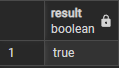
\includegraphics{s6.png}}
		\caption{Результат запроса s6}
	\end{figure}
	
	Результат выполнения запроса s7 представлен на рисунке~7.
	
	\begin{figure}[H]
		\centering
		\adjustbox{max width=\linewidth}{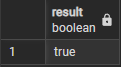
\includegraphics{s7.png}}
		\caption{Результат запроса s7}
	\end{figure}
	
	Результат выполнения запроса s8 представлен на рисунке~8.
	
	\begin{figure}[H]
		\centering
		\adjustbox{max width=\linewidth}{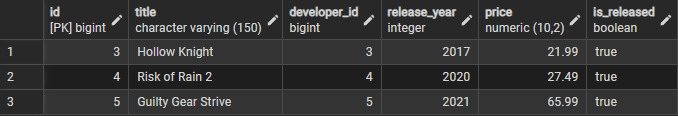
\includegraphics{s8.png}}
		\caption{Результат запроса s8}
	\end{figure}
	
	Результат выполнения запроса s9 представлен на рисунке~9.
	
	\begin{figure}[H]
		\centering
		\adjustbox{max width=\linewidth}{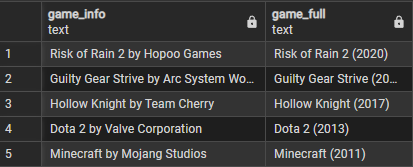
\includegraphics{s9.png}}
		\caption{Результат запроса s9}
	\end{figure}
	
	Результат выполнения запроса s10 представлен на рисунке~10.
	
	\begin{figure}[H]
		\centering
		\adjustbox{max width=\linewidth}{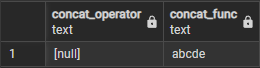
\includegraphics{s10.png}}
		\caption{Результат запроса s10}
	\end{figure}
	
	Результат выполнения запроса s11 представлен на рисунке~11.
	
	\begin{figure}[H]
		\centering
		\adjustbox{max width=\linewidth}{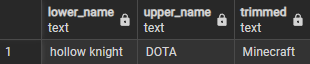
\includegraphics{s11.png}}
		\caption{Результат запроса s11}
	\end{figure}
	
	Результат выполнения запроса s12 представлен на рисунке~12.
	
	\begin{figure}[H]
		\centering
		\adjustbox{max width=\linewidth}{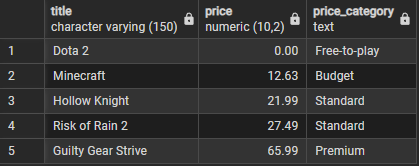
\includegraphics{s12.png}}
		\caption{Результат запроса s12}
	\end{figure}
	
	Результат выполнения запроса s13 представлен на рисунке~13.
	
	\begin{figure}[H]
		\centering
		\adjustbox{max width=\linewidth}{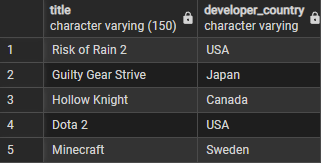
\includegraphics{s13.png}}
		\caption{Результат запроса s13}
	\end{figure}
	
	Результат выполнения запроса s14 представлен на рисунке~14.
	
	\begin{figure}[H]
		\centering
		\adjustbox{max width=\linewidth}{
\includegraphics{s14.png}}
		\caption{Результат запроса s14}
	\end{figure}
	
	Результат выполнения запроса s15 представлен на рисунке~15.
	
	\begin{figure}[H]
		\centering
		\adjustbox{max width=\linewidth}{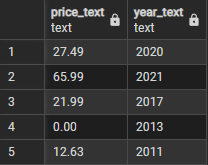
\includegraphics{s15.png}}
		\caption{Результат запроса s15}
	\end{figure}
	
	\newpage
	
	\section*{Работа с датами}
	
	\begin{lstlisting}
		-- s16: текущая дата и время
		SELECT now() AS current_timestamp;
		
		-- s17: преобразование строки в дату
		SELECT 
		to_date('15-03-2024', 'DD-MM-YYYY') AS parsed_date,
		to_timestamp('15-03-2024 14:30', 'DD-MM-YYYY HH24:MI') AS parsed_ts;
		
		-- s18: прибавление интервалов к датам
		SELECT 
		review_date,
		review_date + interval '1 year' AS plus_year,
		review_date - interval '30 day' AS minus_month
		FROM lab_schema.review
		LIMIT 3;
		
		-- s19: возраст игры в годах
		SELECT 
		g.title,
		g.release_year,
		extract(year FROM age(now(), 
		to_date(g.release_year::text || '-01-01', 'YYYY-MM-DD'))) AS years_old
		FROM lab_schema.game g;
		
		-- s20: разница между датами в днях
		SELECT 
		max(review_date) - min(review_date) AS days_between_reviews
		FROM lab_schema.review;
	\end{lstlisting}
	
	Результат выполнения запроса s16 представлен на рисунке~16.
	
	\begin{figure}[H]
		\centering
		\adjustbox{max width=\linewidth}{
\includegraphics{s16.png}}
		\caption{Результат запроса s16}
	\end{figure}
	
	Результат выполнения запроса s17 представлен на рисунке~17.
	
	\begin{figure}[H]
		\centering
		\adjustbox{max width=\linewidth}{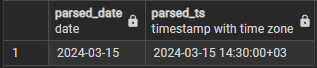
\includegraphics{s17.png}}
		\caption{Результат запроса s17}
	\end{figure}
	
	Результат выполнения запроса s18 представлен на рисунке~18.
	
	\begin{figure}[H]
		\centering
		\adjustbox{max width=\linewidth}{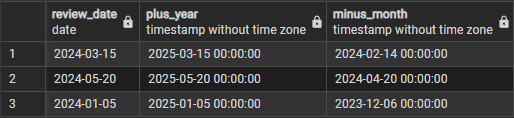
\includegraphics{s18.png}}
		\caption{Результат запроса s18}
	\end{figure}
	
	Результат выполнения запроса s19 представлен на рисунке~19.
	
	\begin{figure}[H]
		\centering
		\adjustbox{max width=\linewidth}{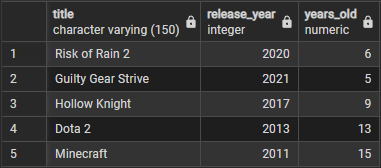
\includegraphics{s19.png}}
		\caption{Результат запроса s19}
	\end{figure}
	
	Результат выполнения запроса s20 представлен на рисунке~20.
	
	\begin{figure}[H]
		\centering
		\adjustbox{max width=\linewidth}{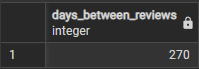
\includegraphics{s20.png}}
		\caption{Результат запроса s20}
	\end{figure}
	
	\newpage
	
	\section*{Подзапросы и предложение WITH}
	
	\begin{lstlisting}
		-- s21: подзапрос в WHERE
		SELECT title, price 
		FROM lab_schema.game 
		WHERE developer_id = (SELECT id FROM lab_schema.developer 
		WHERE name = 'Valve Corporation');
		
		-- s22: подзапрос с IN
		SELECT title 
		FROM lab_schema.game 
		WHERE id IN (SELECT game_id FROM lab_schema.review WHERE score >= 9);
		
		-- s23: WITH (CTE) - статистика разработчиков
		WITH developer_stats AS (
		SELECT 
		d.id,
		d.name AS developer,
		count(g.id) AS games_count,
		round(avg(r.score), 2) AS avg_score
		FROM lab_schema.developer d
		LEFT JOIN lab_schema.game g ON g.developer_id = d.id
		LEFT JOIN lab_schema.review r ON r.game_id = g.id
		GROUP BY d.id, d.name
		)
		SELECT * FROM developer_stats 
		WHERE games_count > 0 
		ORDER BY avg_score DESC NULLS LAST;
		
		-- s24: WITH с несколькими CTE
		WITH expensive_games AS (
		SELECT id, title, price 
		FROM lab_schema.game 
		WHERE price > 20
		),
		high_rated AS (
		SELECT game_id, avg(score) AS avg_score 
		FROM lab_schema.review 
		GROUP BY game_id 
		HAVING avg(score) >= 9
		)
		SELECT eg.title, eg.price, hr.avg_score
		FROM expensive_games eg
		JOIN high_rated hr ON eg.id = hr.game_id;
	\end{lstlisting}
	
	Результат выполнения запроса s21 представлен на рисунке~21.
	
	\begin{figure}[H]
		\centering
		\adjustbox{max width=\linewidth}{
\includegraphics{s21.png}}
		\caption{Результат запроса s21}
	\end{figure}
	
	Результат выполнения запроса s22 представлен на рисунке~22.
	
	\begin{figure}[H]
		\centering
		\adjustbox{max width=\linewidth}{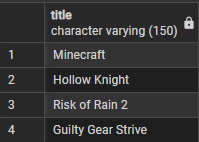
\includegraphics{s22.png}}
		\caption{Результат запроса s22}
	\end{figure}
	
	Результат выполнения запроса s23 представлен на рисунке~23.
	
	\begin{figure}[H]
		\centering
		\adjustbox{max width=\linewidth}{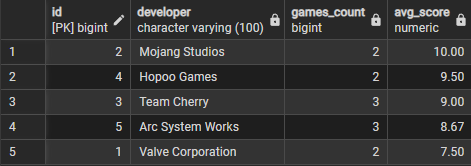
\includegraphics{s23.png}}
		\caption{Результат запроса s23}
	\end{figure}
	
	Результат выполнения запроса s24 представлен на рисунке~24.
	
	\begin{figure}[H]
		\centering
		\adjustbox{max width=\linewidth}{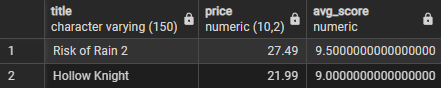
\includegraphics{s24.png}}
		\caption{Результат запроса s24}
	\end{figure}
	
	\newpage
	
	\section*{Предложение RETURNING}
	
	\begin{lstlisting}
		-- s25: INSERT с RETURNING
		INSERT INTO lab_schema.developer (name, country, is_active)
		VALUES ('FromSoftware', 'Japan', true)
		RETURNING id, name, country;
		
		-- s26: UPDATE с RETURNING
		UPDATE lab_schema.game
		SET price = price * 0.9
		WHERE title = 'Minecraft'
		RETURNING title, price AS new_price;
		
		-- s27: DELETE с RETURNING
		DELETE FROM lab_schema.developer
		WHERE name = 'FromSoftware'
		RETURNING *;
		
		-- s28: WITH + RETURNING для вставки связанных данных
		WITH new_dev AS (
		INSERT INTO lab_schema.developer (name, country, is_active)
		VALUES ('Test Studio', 'USA', true)
		RETURNING id
		)
		INSERT INTO lab_schema.game (title, developer_id, release_year, price, is_released)
		SELECT 'Test Game', id, 2025, 19.99, true
		FROM new_dev
		RETURNING *;
		
		-- Очистка тестовых данных
		DELETE FROM lab_schema.game WHERE title = 'Test Game';
		DELETE FROM lab_schema.developer WHERE name = 'Test Studio';
	\end{lstlisting}
	
	Результат выполнения запроса s25 представлен на рисунке~25.
	
	\begin{figure}[H]
		\centering
		\adjustbox{max width=\linewidth}{
\includegraphics{s25.png}}
		\caption{Результат запроса s25}
	\end{figure}
	
	Результат выполнения запроса s26 представлен на рисунке~26.
	
	\begin{figure}[H]
		\centering
		\adjustbox{max width=\linewidth}{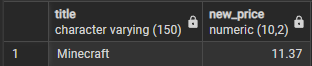
\includegraphics{s26.png}}
		\caption{Результат запроса s26}
	\end{figure}
	
	Результат выполнения запроса s27 представлен на рисунке~27.
	
	\begin{figure}[H]
		\centering
		\adjustbox{max width=\linewidth}{
\includegraphics{s27.png}}
		\caption{Результат запроса s27}
	\end{figure}
	
	Результат выполнения запроса s28 представлен на рисунке~28.
	
	\begin{figure}[H]
		\centering
		\adjustbox{max width=\linewidth}{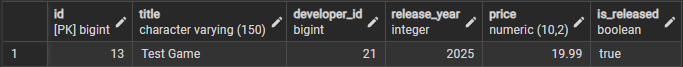
\includegraphics{s28.png}}
		\caption{Результат запроса s28}
	\end{figure}
	
	\newpage
	
	\section*{Планы выполнения запросов (EXPLAIN) и FORMAT JSON}
	
	\begin{lstlisting}
		-- s29: простой EXPLAIN
		EXPLAIN SELECT * FROM lab_schema.game;
		
		-- s30: EXPLAIN с ANALYZE
		EXPLAIN (ANALYZE) SELECT * FROM lab_schema.game WHERE price > 20;
		
		-- s31: EXPLAIN с BUFFERS
		EXPLAIN (ANALYZE, BUFFERS) 
		SELECT * FROM lab_schema.review WHERE score >= 9;
		
		-- s32: EXPLAIN FORMAT JSON для простого соединения
		EXPLAIN (FORMAT JSON) SELECT * FROM lab_schema.game 
		JOIN lab_schema.developer ON game.developer_id = developer.id;
		
		-- s33: EXPLAIN FORMAT JSON для сложного запроса
		EXPLAIN (FORMAT JSON, ANALYZE)
		SELECT g.title, d.name, string_agg(gen.name, ', ') AS genres
		FROM lab_schema.game g
		JOIN lab_schema.developer d ON g.developer_id = d.id
		JOIN lab_schema.game_genre gg ON g.id = gg.game_id
		JOIN lab_schema.genre gen ON gg.genre_id = gen.id
		GROUP BY g.id, g.title, d.name;
	\end{lstlisting}
	
	Результат выполнения запроса s29 представлен на рисунке~29.
	
	\begin{figure}[H]
		\centering
		\adjustbox{max width=\linewidth}{
\includegraphics{s29.png}}
		\caption{Результат запроса s29}
	\end{figure}
	
	Результат выполнения запроса s30 представлен на рисунке~30.
	
	\begin{figure}[H]
		\centering
		\adjustbox{max width=\linewidth}{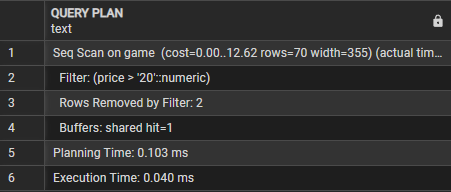
\includegraphics{s30.png}}
		\caption{Результат запроса s30}
	\end{figure}
	
	Результат выполнения запроса s31 представлен на рисунке~31.
	
	\begin{figure}[H]
		\centering
		\adjustbox{max width=\linewidth}{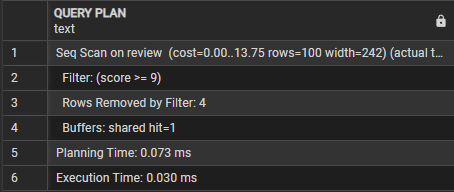
\includegraphics{s31.png}}
		\caption{Результат запроса s31}
	\end{figure}
	
	Результат выполнения запроса s32 представлен на рисунке~32.
	
	\begin{figure}[H]
		\centering
		\adjustbox{max width=\linewidth}{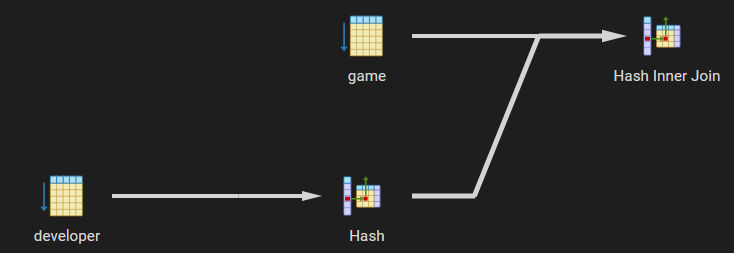
\includegraphics{s32.png}}
		\caption{Результат запроса s32}
	\end{figure}
	
	Результат выполнения запроса s33 представлен на рисунке~33.
	
	\begin{figure}[H]
		\centering
		\adjustbox{max width=\linewidth}{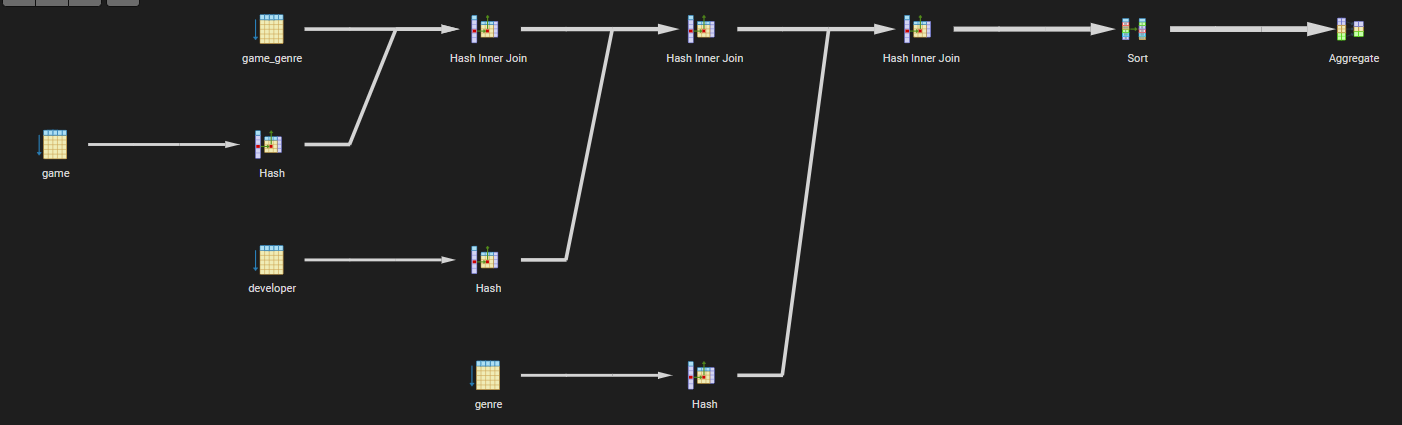
\includegraphics{s33.png}}
		\caption{Результат запроса s33}
	\end{figure}
	
	\newpage
	
	\section*{Сравнение трёх способов соединения}
	
	Для одного и того же запроса были выполнены три способа соединения наборов строк: вложенный цикл (Nested Loop), хеширование (Hash Join) и слияние (Merge Join).
	
	\begin{lstlisting}
		-- s34: Nested Loop (вложенный цикл)
		SET enable_mergejoin = off;
		SET enable_hashjoin = off;
		EXPLAIN (ANALYZE, FORMAT JSON)
		SELECT g.title, d.name AS developer, r.score
		FROM lab_schema.game g
		JOIN lab_schema.developer d ON g.developer_id = d.id
		JOIN lab_schema.review r ON r.game_id = g.id;
		SET enable_mergejoin = on;
		SET enable_hashjoin = on;
		
		-- s35: Hash Join (хеширование)
		SET enable_nestloop = off;
		SET enable_mergejoin = off;
		EXPLAIN (ANALYZE, FORMAT JSON)
		SELECT g.title, d.name AS developer, r.score
		FROM lab_schema.game g
		JOIN lab_schema.developer d ON g.developer_id = d.id
		JOIN lab_schema.review r ON r.game_id = g.id;
		SET enable_nestloop = on;
		SET enable_mergejoin = on;
		
		-- s36: Merge Join (слияние)
		SET enable_nestloop = off;
		SET enable_hashjoin = off;
		EXPLAIN (ANALYZE, FORMAT JSON)
		SELECT g.title, d.name AS developer, r.score
		FROM lab_schema.game g
		JOIN lab_schema.developer d ON g.developer_id = d.id
		JOIN lab_schema.review r ON r.game_id = g.id;
		SET enable_nestloop = on;
		SET enable_hashjoin = on;
	\end{lstlisting}
	
	Результат выполнения запроса s34 (Nested Loop) представлен на рисунке~34.
	
	\begin{figure}[H]
		\centering
		\adjustbox{max width=\linewidth}{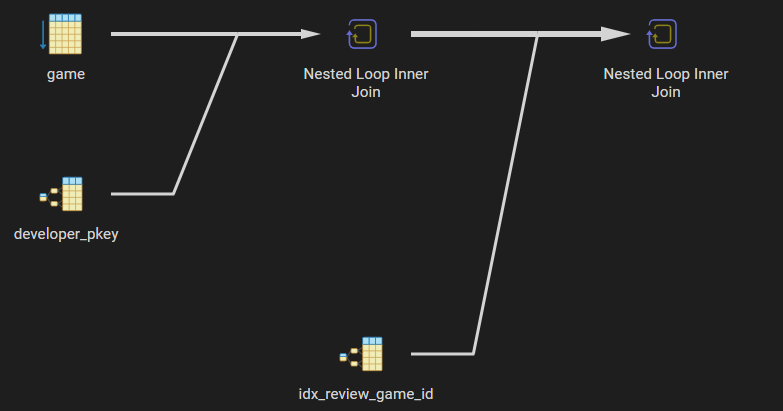
\includegraphics{s34.png}}
		\caption{Результат запроса s34 (Nested Loop)}
	\end{figure}
	
	Результат выполнения запроса s35 (Hash Join) представлен на рисунке~35.
	
	\begin{figure}[H]
		\centering
		\adjustbox{max width=\linewidth}{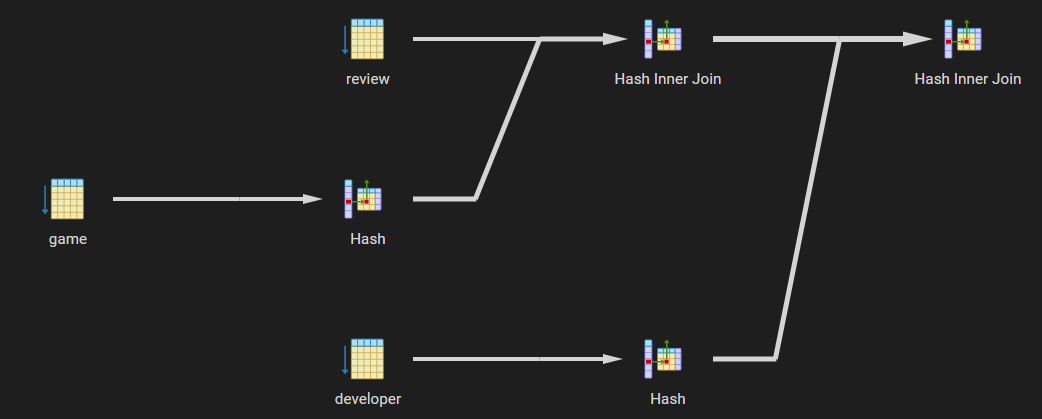
\includegraphics{s35.png}}
		\caption{Результат запроса s35 (Hash Join)}
	\end{figure}
	
	Результат выполнения запроса s36 (Merge Join) представлен на рисунке~36.
	
	\begin{figure}[H]
		\centering
		\adjustbox{max width=\linewidth}{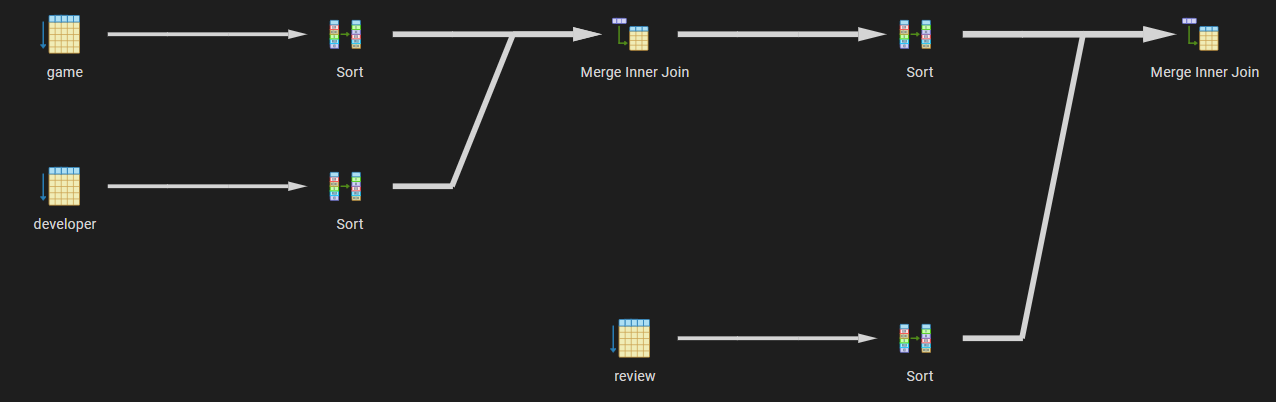
\includegraphics{s36.png}}
		\caption{Результат запроса s36 (Merge Join)}
	\end{figure}
	
	Анализ планов выполнения показал, что для данной выборки на небольших объёмах данных наиболее оптимальным является метод Nested Loop, так как он имеет наименьшую фактическую стоимость выполнения. Для больших объёмов данных предпочтительнее использовать Hash Join, а Merge Join эффективен при предварительно отсортированных наборах данных.
	
	\newpage
	
	\section*{Выводы} В ходе выполнения лабораторной работы были освоены агрегатные функции (count, sum, avg, min, max, string\_agg) и предложения GROUP BY и HAVING для группировки данных. Изучены операторы и встроенные функции PostgreSQL: логические операторы, конкатенация строк, функции работы с регистром, LIKE для поиска по шаблону, CASE и COALESCE для условной выборки, приведение типов через оператор ::. Освоена работа с датами: функции now(), to\_date(), to\_timestamp(), операции с временными интервалами (interval) и вычисление разницы между датами. Изучены подзапросы и предложение WITH (CTE) для создания именованных общих табличных выражений. Освоено предложение RETURNING для получения результатов операций INSERT, UPDATE и DELETE. Рассмотрены планы выполнения запросов с помощью команды EXPLAIN с различными параметрами (ANALYZE, BUFFERS, FORMAT JSON). Выполнены три способа соединения наборов строк (Nested Loop, Hash Join, Merge Join) для одной и той же выборки и определён наиболее оптимальный метод для заданных условий.
	
\end{document}